\documentclass[12pt]{article}

\usepackage[utf8]{inputenc}
\usepackage{latexsym,amsfonts,amssymb,amsthm,amsmath}
\usepackage {tikz}
\usetikzlibrary {positioning}

\setlength{\parindent}{0in}
\setlength{\oddsidemargin}{0in}
\setlength{\textwidth}{6.5in}
\setlength{\textheight}{8.8in}
\setlength{\topmargin}{0in}
\setlength{\headheight}{18pt}

\definecolor {processblue}{cmyk}{0.96,0,0,0}

\title{Graph Theory - Homework 1}
\author{Kishlaya Jaiswal}

\begin{document}

\maketitle

\vspace{0.5in}


\subsection*{Exercise 1}
\begin{proof}
Since $G$ is not connected, there are atleast two non-empty disconnected components.

Let $u$ and $v$ be two vertices in $\bar{G}$. 

\textbf{Case 1}: If $u$ and $v$ are in different connected components in $G$, then there is an edge $(u,v) \in \bar{G}$ and so there is a path between $u$ and $v$ in $\bar{G}$

\textbf{Case 2}: If $u$ and $v$ are in same connected component in $G$. Consider $w$ in a separate connected component of $G$. Hence there are edges $(u,w)$ and $(v,w)$ in $\bar{G}$. Hence, $u \rightarrow w \rightarrow v$ is a path between $u$ and $v$ in $\bar{G}$.
\end{proof}

\newpage
\subsection*{Exercise 2}
\begin{proof}
\textbf{Case:} $n=3$
\begin{center}
\begin{tikzpicture}[shorten >=1pt,->]
  \tikzstyle{vertex}=[circle ,top color =white , bottom color = processblue!20 ,
draw,processblue , text=blue , minimum width =1 cm]
  \node[vertex] (G_1) at (0,0) {1};
  \node[vertex] (G_2) at (-3,-3)   {2};
  \node[vertex] (G_3) at (-3,-6)  {3};
  \node[vertex] (G_4) at (0,-9)  {4};
  \node[vertex] (G_5) at (3,-6)  {5};
  \node[vertex] (G_6) at (3,-3)  {6};
  \draw (G_1) -- (G_2) -- (G_3) -- (G_4) -- (G_5) -- (G_6) -- (G_1) -- cycle;
  \draw (G_1) -- (G_4) -- cycle;
  \draw (G_2) -- (G_5) -- cycle;
  \draw (G_3) -- (G_6) -- cycle;
\end{tikzpicture}
\end{center}

\newpage
\textbf{Case:} $n > 3$
\begin{center}
\begin{tikzpicture}[shorten >=1pt,->]
  \tikzstyle{vertex}=[circle ,top color =white , bottom color = processblue!20 ,
draw,processblue , text=blue , minimum width =1 cm]
  \node[vertex] (G_1) at (0,5) {1};
  \node[vertex] (G_2) at (2.5,4.33)   {2};
  \node[vertex] (G_3) at (4.33,2.5)  {3};
  \node[vertex] (G_4) at (5,0)  {4};
  \node[vertex] (G_5) at (4.33,-2.5)  {5};
  \node[vertex] (G_6) at (2.5,-4.33)   {6};
  \node[vertex] (G_7) at (0,-5)   {7};
  \node[vertex] (G_8) at (-2.5,-4.33)   {8};
  \node[vertex] (G_n) at (-2.5,4.33)   {n};
  \node[vertex] (G_n1) at (-4.33,2.5)  {n-1};
  \draw (G_1) -- (G_2) -- (G_3) -- (G_4) -- (G_5) -- (G_6) -- (G_7) -- (G_8) -- cycle;
  \draw [dashed] (G_8) -- (-4.33,-2.5) -- (-5,0) -- (G_n1) -- cycle;
  \draw (G_n1) -- (G_n) -- (G_1) -- cycle;
  
  \node[vertex] (H_1) at (0,7) {n+1};
  \node[vertex] (H_2) at (3.5,6.06)   {n+2};
  \node[vertex] (H_3) at (6.06,3.5)  {n+3};
  \node[vertex] (H_4) at (7,0)  {n+4};
  \node[vertex] (H_5) at (6.06,-3.5)  {n+5};
  \node[vertex] (H_6) at (3.5,-6.06)   {n+6};
  \node[vertex] (H_7) at (0,-7)   {n+7};
  \node[vertex] (H_8) at (-3.5,-6.06)   {n+8};
  \node[vertex] (H_n) at (-3.5,6.06)   {2n};
  \node[vertex] (H_n1) at (-6.06,3.5)  {2n-1};
  \draw (H_1) -- (H_2) -- (H_3) -- (H_4) -- (H_5) -- (H_6) -- (H_7) -- (H_8) -- cycle;
  \draw [dashed] (H_8) -- (-6.06,-3.5) -- (-7,0) -- (H_n1) -- cycle;
  \draw (H_n1) -- (H_n) -- (H_1) -- cycle;
  
  \draw (G_1) -- (H_1) -- cycle;
  \draw (G_2) -- (H_2) -- cycle;
  \draw (G_3) -- (H_3) -- cycle;
  \draw (G_4) -- (H_4) -- cycle;
  \draw (G_5) -- (H_5) -- cycle;
  \draw (G_6) -- (H_6) -- cycle;
  \draw (G_7) -- (H_7) -- cycle;
  \draw (G_8) -- (H_8) -- cycle;
  \draw (G_n1) -- (H_n1) -- cycle;
  \draw (G_n) -- (H_n) -- cycle;
\end{tikzpicture}
\end{center}

Here is a more general construction for \textbf{$k-$regular graphs on $2n$ vertices, which contain no odd cycles}.

Let $G = (U \cup V, E)$ where $U=\{u_0,u_2,\ldots u_{n-1}\}$ and $V=\{v_0,v_2,\ldots v_{n-1}\}$ and $E = \{\{u_i,v_j\} \mid 0 \leq i \leq n-1, i \leq j \leq  i+k-1 \pmod n\}$

This is clearly $k-regular$ and it doesn't have any odd cycles because it is a bipartite graph.

\end{proof}

\newpage
\subsection*{Exercise 3}
We shall prove the following stronger assertion: If a graph $G$ has exactly two no-cut-vertices, then $G$ is a path.
\begin{proof}
Let $P$ be an arbitrary maximal path in $G$ and let $a$ and $b$ be its endpoints.

(Note that all neighbours of $a$ and $b$ lie on $P$ by maximality of $P$)

We claim that $a$ and $b$ are no-cut vertices. For that let $C$ be the connected component containing $a$ and $b$. Now consider any $x,y  \in C$. We will show that there is a path connecting $x,y$ such that $a, b$ do not lie on this path. So let $Q$ be any path joining $x,y$. If $a \in Q$, say $Q = x \ldots vav' \ldots y$ then since $v,v' \in N(a)$, we know from above reasoning that $v,v' \in P$ and so we can eliminate $a$ from $Q$. Similar argument holds for $b$. Therefore, $a,b$ are no-cut vertices.

But $G$ has exactly two no-cut vertices, so $G$ must be connected because for $v \in G$, let $P_v$ be a maximal path passing through $v$. So, $a$ and $b$ must be the end-points of $P_v$ and hence every vertex $v$ lies in $C$ (connected component of $a,b$).

Now we claim that $G = P$. Suppose there is a vertex $x \not \in P$. Hence $x$ is a cut vertex. So, $G \setminus \{x\}$ has atleast two connected components. Clearly, $a$ and $b$ still lie in the same connected component. But choose any $y$ from the other connected component of $G \setminus \{x\}$ and let $P_y$ be maximal path containing $y$ in $G$. Then $P_y = Q_aQ_b$ where $Q_a = a \ldots y$ and $Q_b = y \ldots b$. Since $y$ is in a different connected component, $x \in P_y$. If $x \in Q_a$ then path $Q_b$ is still a path in $G \setminus \{x\}$ which means $y$ is the same connected component as $b$, which is a contradiction. Similarly, if $x \in Q_b$ then $y$ is in the same connected component as $a$, which is again a contradiction. 

Furthermore, let $P = av_1v_2 \ldots v_k$ then there cannot be any extra edge like $\{v_i, v_j\}$ because otherwise $v_{i+1}$ will be a cut vertex. Hence $G=P$.

\end{proof}

\subsection*{Exercise 4}
\begin{proof}
$$2|E| = \sum_v d(v) \geq 2n \implies |E| \geq n$$

We know that a tree has exactly $n-1$ edges.

Since $G$ is connected and has more than $n-1$ edges, $G$ contains a cycle.

This is not true if the graph $G$ is infinite. For example, consider the two-sided infinite path $G = (V,E)$ where $V = \mathbb{Z}$ and $E = \{\{i,i+1\} \mid i \in \mathbb{Z}\}$
\end{proof}

\vspace{2in} %Leave more space for comments!



\end{document}

